\documentclass{article}
\usepackage[margin=1in]{geometry}
\usepackage{graphicx}
\usepackage{hyperref,fancyvrb,amsmath}
\usepackage{tikz}

\newcommand{\mydot}[1]{\draw[fill] (#1) circle (0.1);}

\title{CSCI 241, Project \#2, Raytracing Optimization}
\author{Geoffrey Matthews}

\begin{document}

\maketitle

\centerline{\bf Note:  This is still incomplete.}

\centerline{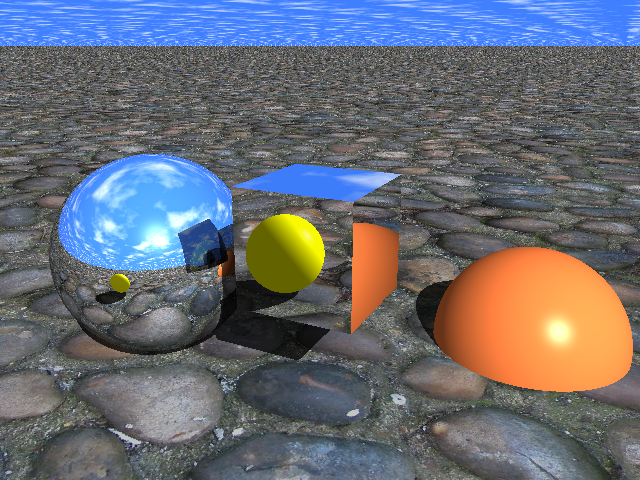
\includegraphics[scale=0.5]{testmain.png}}

\begin{description}

\item[Due date:] Midnight, May 12.

\item[Ray tracing:]
Ray tracing is a fairly direct method of making spectacularly
realistic images on the computer.  The image above is one I made to
demonstrate what was possible for the first project in CSCI 480 one
year.  One of the major problems with raytracing is that it is very
slow. 

We won't be including all the features that made the above image
possible, we will only be rendering simple spheres.  But we will use a
tree structure to improve the speed of the rendering.


  \begin{figure}
\centerline{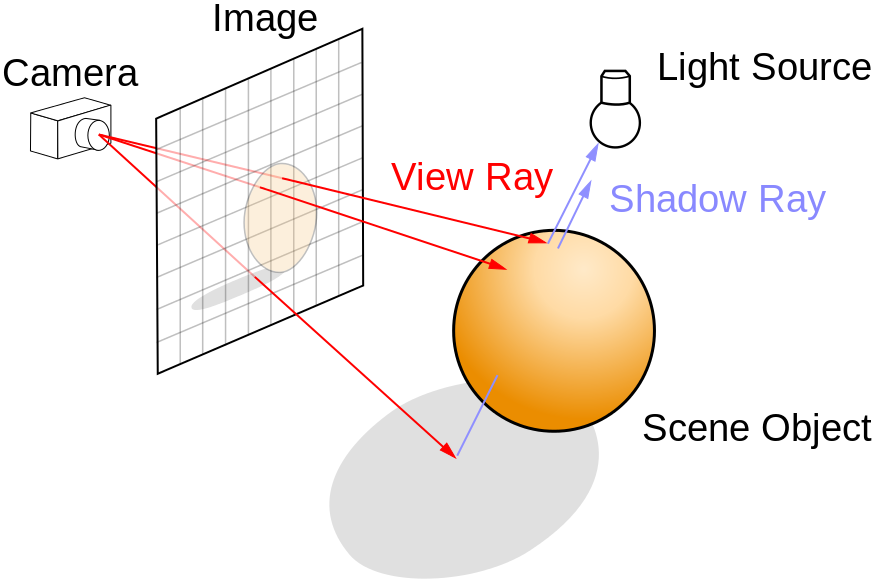
\includegraphics[scale=0.25]{Ray_trace_diagram.png}}
\caption{Basic world for ray tracing.  We will not be using shadow
  rays.
  (By Henrik - Own work, GFDL,
  \url{https://commons.wikimedia.org/w/index.php?curid=3869326})}
    \label{raytracing}
  \end{figure}

\item[The world:]
  
The world we need to represent (see Figure \ref{raytracing}), consists
of the following things:
\begin{enumerate}
\item{\bf A camera:} This is just a point in space, $p$.  To make the math
  a little simpler, we will assume that this point is on the $z$ axis,
  at point $p=(0,0,d)$. In the program, the constant $d$ will be
  called the \verb|CAMERA_DISTANCE|, and we will assume $d > 0$.
\item{\bf An image plane:} This is a flat rectangular region of space in
  front of the camera.  Each grid point on the image plane will
  determine a color for a pixel in the image.  To simplify the math,
  again, we will assume our image plane is a square centered in the
  $(x,y)$ plane, so that its corners are at $(\pm s , \pm s, 0)$.  In
  the program, the constant $s$ will be called the
  \verb|IMAGE_PLANE_ZIZE|.
\item{\bf A light source:} We will assume only one light source, and we
  will assume that it is so distant, that it appears to be in the same
  direction no matter where you are in the world.  It will be
  represented, therefore, by a single 3d vector, $\ell =
  (\ell_x,\ell_y,\ell_z)$.  convenience, we assume the vector is {\em
    normalized}, that is, it's length is one: $\sqrt{\ell_x^2 +
    \ell_y^2 + \ell_z^2} = 1$.  For example, one light source could be
  $\ell = (1/\sqrt{3},1/\sqrt{3},1/\sqrt{3})$.  In the program, the
  light will be represented by the constant \verb|LIGHT|.
\item{\bf Objects:} Objects in the scene to be rendered.  For our
  purposes, the only objects we will render will be {\em spheres},
  which are represented by a data structure that holds a 3D point for
  the center, $c$, and a real number $r$, for the radius.  We will
  want to include many spheres, so you will need to use some kind of a
  container for the spheres.  A linear structure is fine, since we
  will just be iterating over them.

  Spheres will also have a {\em color}, which will be a vector of
  three floats giving the red, green, and blue components of the color
  of the sphere.
\end{enumerate}


\item[Pseudocode:]\mbox{}
  
\begin{Verbatim}[frame=single,numbers=left]
  for each pixel in the image {
    find the ray from the camera
    for each sphere in the world {
      intersect the ray with the sphere
      keep the closest sphere and intersection point (largest z-value)
    }
    if there were no intersections {
      put the background color in the pixel
    } else {
      color the pixel with Lambertian shading of the intersection point
    }
  }
\end{Verbatim}    

\item[Explanation of pseudocode:]\mbox{}
  
  \begin{description}
  \item Line 1.  We open our Java
     image with a size of \verb|WIDTH| $=w$ and
    \verb|HEIGHT| $=h$, and 
    we iterate over the pixels in our
    image with the variables $u$ and $v$, with
    $u=0\ldots w-1$
    and $v=0\ldots h-1$.
  \item Line 2. In order to make a 2D image from our 3D world, we need
    to map pixels in the 2D image to points in the image plane.  
    The integer pixel $(u,v)$ will be mapped to the
    following 3D point on the image plane, with
    $s=$ \verb|IMAGE_PLANE_SIZE|: 
    \begin{eqnarray*}
    \mbox{image\_plane}(u,v) &=&
    (s(2u/w-1), -s(2v/h-1), 0)\\
    &=& q
    \end{eqnarray*}

    The {\bf ray} from the camera point $p$ through a point $q$ on the
    image plane, is a data structure that consists of the camera
    point and a vector, $(p,v)$, where $v$ is the {\em normalized} vector
    \[
    v = \frac{q-p}{|q-p|}
    \]

  \item Line 3.  Let us assume that, as we loop through the sphere
    objects, $(c,r)$ is the current sphere we're talking about.

  \item Line 4.    
    Given a ray, $(p,v)$  and a sphere $(c,r)$,
    we can find the intersection point as
follows (refer to Figure \ref{intersectingraysphere}).
We need to solve the equation, for some value of $t$
(skip the math if you're not interested):
\[
|p + tv|^2 = r^2
\]
We can do this as follows.
\begin{eqnarray*}
|p+tv|^2 &=& (p+tv)\cdot(p+tv)\\
&=& \sum_i (p_i + tv_i)(p_i + tv_i)\\
&=& \sum_i \left(p_i^2 + 2p_iv_it + v_i^2t^2\right)\\
&=& \sum_i p_i^2 + 2\sum_ip_iv_it + \sum_iv_i^2t^2\\
&=& (p\cdot p) + 2(p\cdot v) t+ (v\cdot v) t^2
\end{eqnarray*}
So, in the quadratic $at^2 + bt + c = 0$,
\begin{eqnarray*}
a &=& v\cdot v \ \ \ (= 1, \mbox{why?})\\
b &=& 2p\cdot v\\
c &=& p\cdot p - r^2
\end{eqnarray*}
The two solutions to this quadratic will give you two values of $t$ to
plug into the expression
\[
p + tv
\]
where $(p,v)$ is your ray.  This will give you the two intersection
points on the sphere, as in Figure \ref{intersectingraysphere}.  Pick
the one closest to the camera; it will have the smallest $t$ value
(why?).

\begin{figure}

    \begin{center}
    \begin{tikzpicture}[scale=0.5,>=latex,thick]
      \draw (5,4) node[anchor=north east] {$c$} circle (4);
      \draw[dotted] (-10,0) -- (10,8);
      \draw[arrows=->] (-10,0) -- (-5,2) node[anchor=north] {$v$};
      \draw[fill] (-10,0) node[anchor=north] {$p$} circle (0.1);
      \mydot{5,4}
      \draw (5,4) -- (9,4);
      \draw (7,4) node[anchor=north] {$r$};
      \mydot{1,4.4}
      \mydot{7.6,7}
    \end{tikzpicture}
\end{center}    

    \caption{Intersecting a ray and a sphere.}
    \label{intersectingraysphere}
\end{figure}


\item Line 5.  The closest intersection point will have the largest
  $z$ value (why?).

\item Line 10.
 If we use the
sphere's color for this pixel, we get a figure like the one in Figure
\ref{spheresflat}.  This is not very exciting.  We would like to shade
the spheres as in Figure \ref{sphereslambertian}.

\begin{figure}
  \centerline{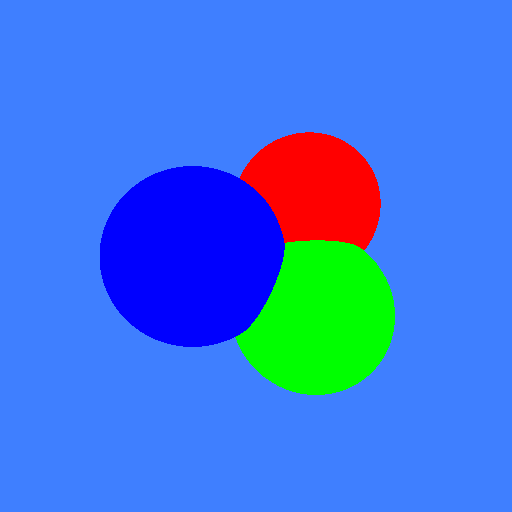
\includegraphics[scale=0.5]{threeflatspheres.png}}
  \caption{Three spheres, flat shading.}
  \label{spheresflat}
\end{figure}

\begin{figure}
  \centerline{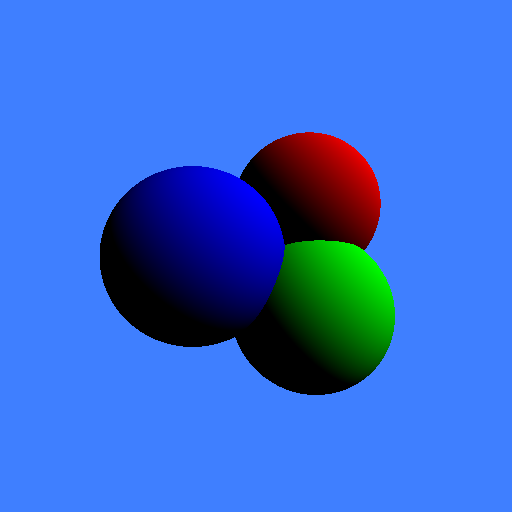
\includegraphics[scale=0.5]{threelambertianspheres.png}}
  \caption{Three spheres, Lambertian shading.}
  \label{sphereslambertian}
\end{figure}

We will use {\em Lambertian shading}
for the spheres, a very simple shader.
We just have to multiply the
color of the sphere by the cosine of the angle between the surface
normal, $n$, and the light vector, $\ell$.  This is easier than it sounds.

To find the surface normal, $n$, of a sphere, $(c,r)$ at any point, $p$,
simply subtract the center from the point and normalize the
resulting vector:
\[
n = \mbox{normalize}(p-c)
\]
To find the cosine of the angle between two normalized vectors, simply
take the dot product.
\[
\cos(\mbox{angle}(n,\ell)) = n \cdot \ell
\]
In this case, if the cosine is negative, we want the color to be
black, so any result that is negative is replaced with zero.
We then multiply the color of the sphere by this value (between 0 and
1), to get the shading seen in Figure \ref{sphereslambertian}.

If you want to get a little bit of color in the shadows (instead of
pitch black), you can truncate the cosine at a small number, say 0.1,
instead of 0, to add some {\em diffuse} shading.

Note that this only works if both $n$ and $\ell$ are normalized.

  \end{description}
  

\item[Java code for images:]
  I found the simplest Java code I could on the web to create an image
  and color its pixels.  This file, called {\tt Example01.java} is on
  the website.  It should be self-explanatory.

  Given the pseudocode above and the Java example, you should be able
  to make some pretty amazing pictures (such as the ones at the end of
  this document).

  Don't put the camera too close to the scene, unless you want
  extremely exaggerated perspective.  Place all the spheres near the
  image plane (in the $(\pm s, \pm s, \pm s)$ cube), or you won't see
  them in the image.

\item[World files:]  Input to this program will be the description of
  a world.  Output will simply be the graphical display.

  The world description will be in a file, which will give the camera
  position, the light direction, and the spheres.  Here is an example
  world file, it puts the camera at 20 units along the $z$ axis, the
  light at $\mbox{normalized(1,1,1)}$, and a red sphere of radius 3 at
  $(2,2,-1)$, a green sphere of radius 3 at $(2,-2,0)$, and a blue
  sphere of radius 2 at $(-2,0,1)$.

  \begin{Verbatim}[frame=single,label=myworld.wrl]
camera: 20
light: 0.577 0.577 0.577
sphere:  2.0  2.0 -1.0 3.0 1.0 0.0 0.0
sphere:  2.0 -2.0  0.0 3.0 0.0 1.0 0.0
sphere: -2.0  0.0  1.0 2.0 0.0 0.0 1.0
\end{Verbatim}

\item[Optimizing the ray tracing:]  This is done in two phases,
  calculating the bounding boxes for the spheres, and then inserting
  the spheres into a tree.

  \begin{description}
    \item[Bounding boxes:]
  The method described so far is easy to implement and will create
  stunning images of spheres.  However, it is not very efficient.  We
  need to cast thousands of rays.  Even a relatively small image of
  size $256\times256$ will have 65536 rays.  Each of these rays is
  intersected with {\em every} sphere in the world.  We can do better.

  Let's see if we can tell in advance whether or not a ray might hit a
  sphere, and eliminate some of these expensive tests.

Our strategy is to find a rectangular region in the image plane such
that, if the ray does {\em not} go through this region, then it's
impossible for the ray to intersect the sphere.  We call this region
the {\em bounding box} for the sphere.  It will consist of an extent
in $x$, from $x_1$ to $x_2$, and an extent in $y$, from $y_1$ to
$y_2$.  If we assume   $x_1 < x_2$ and $y_1 < y_2$ then we can
represent the rectangle by its corners: $(x_1,y_1)$ and $(x_2, y_x)$.  

Let's consider the $y$ extent, first.  Figure \ref{spherebox} is a
picture of a typical sphere viewed in the $(y,z)$ plane.  The camera is
located at point $p$, the sphere at point $c$ with radius $r$.  We
want to find the numbers $y_1$ and $y_2$.



  \begin{figure}
    \begin{center}
    \begin{tikzpicture}[scale=0.6,>=latex,thick]
      \draw[arrows=<->] (-12,0) node[anchor=east] {$z$} -- (10,0);
      \draw[arrows=<->] (0,-3) -- (0,10) node[anchor=south] {$y$};
      \draw (5,4) node[anchor=north east] {$c$} circle (2);
      \draw (-10,0) -- (4.5,5.95);
      \draw (-10,0) -- (5.5,2.025);
      \draw (4.5,5.95) -- (5.5,2.025);
      \draw[dotted] (-10,0) -- (5,4);
      \draw (4.75, 5) node[anchor=west] {$r$};
      \draw[fill] (-10,0) node[anchor=north] {$p$} circle (0.1);
      \draw[fill] (5,4) circle (0.1);
      \draw[fill] (4.5,5.95) circle (0.1);
%      \draw (4.5,5.95) node[anchor=south] {$c_2$};
      \draw[fill] (5.5,2.025) circle (0.1);
%      \draw (5.5,2.025) node[anchor=north] {$c_1$};
      \mydot{0,1.3}
      \draw (0,1.3) node[anchor=south east] {$y_1$};
      \mydot{0,4.1}
      \draw (0,4.1) node[anchor=south east] {$y_2$};
\draw (-2,2) node {$a$};
\draw (-5.9,1.4) node {$\theta$};
\draw (-5.7,0.85) node {$\theta$};
\draw (-5.6,0.25) node {$\phi$};
\draw (-6,0) arc (0:22:4);
    \end{tikzpicture}
    \end{center}
    \caption{Calculating the image plane bounding box of a sphere.
      All rays from 
      the camera at $p$ that intersect the sphere at $c$ with radius
      $r$ must pass through the image plane between $y_1$ and $y_2$.
      A figure for the $(x,z)$ plane is similar.}
    \label{spherebox}
    
  \end{figure}

We can find the numbers $y_1$ and $y_2$ with a little trigonometry.
$a$ is the distance in the $(y,z)$ plane between $p=(0,0,p_z)$ and $c =
(c_x,c_y,c_z)$, 
which is
\[
a = \sqrt{c_y^2 + (c_z - p_z)^2}
\]
And then, since the radii of the circle are perpendicular to it, we
have
\[
\tan(\theta) = \frac{r}{a}
\]
from which we can find $\theta$.  If we let $\psi = \theta+\phi$, then
\[
\sin(\psi) = \frac{c_y}{a}
\]
from which we can get $\psi$, and $\phi = \psi - \theta$.  It's then
easy to conclude that
\begin{eqnarray*}
  y_1 &=& p_z \tan(\phi)\\
  y_2 &=& p_z \tan(\phi + 2\theta)
\end{eqnarray*}
We can do the same thing in the $(x,z)$ plane, getting $x_1$ and $x_2$.

As in the figure, we let $x_1 < x_2$ and $y_1 < y_2$.

For each sphere, then, we have limits on the rays that might hit it.
Each ray that hits the sphere must hit the image plane in the
rectangle between $(x_1,y_1)$ and $(x_2, y_2)$.  If the ray does not
go through this rectangle, we do not have to test the ray against this
sphere for intersection.

When we trace a ray, we find the point at which it intersects the
image plane.  If this point is not in a sphere's bounding box, then
the ray cannot hit it.  We need a way to quickly find all spheres with
bounding boxes that intersect this ray.

\item[Preprocessing the spheres:]
  Prior to beginning our raytrace, we insert each sphere into a quadtree.
  We divide the image plane up into four quadrants: {\em ul}, upper
  left, {\em ur} upper right, {\em ll} lower left, and {\em lr} lower
  right.  We build a tree to represent the entire image plane ($\pm s$
  in the $(x,y)$ plane), and its four children represent the four parts
  of the image plane.

  Clearly, we can then divide each of the four children into four
  parts ({\em ul, ur, ll, lr}), getting a tree with 16 leaves.  If we
  do this one more time, we get a tree with 64 leaves.  This will be
  our optimization tree.  Each 1/64th of the image plane will be
  called a {\em cell}.  Each cell stores its extent in the $(x,y)$
  plane. 

  Before we begin the raytracing, we insert each sphere into the
  quadtree.  We insert a sphere in a subtree when its bounding box
  intersects the extent of the subtree.
  If we begin inserting at the top, we can reach a leaf in
  only $\log_2 64 = 4$ steps!  Bear in mind, however, that a circle
  may intersect more than one quadrant at each level.  Simply insert
  it into every quadrant its bounding box intersects.

  When we construct a ray, we know which point of the image plane it
  hits.  We can quickly traverse the tree to find the cell that the
  ray hits.  We retrieve its accompanying list of spheres and we test
  the ray for intersection with each one of these, instead of the
  entire list of spheres.

  What kind of speedup can we expect?  If there are large empty areas
  of your scene (as in many scenes), the speedup will be huge.  Any
  ray in these areas will not be tested against {\em any spheres}.  As
  the spheres get more dense, or larger, the speedup may not be so
  great. 

  We can, of course, use deeper trees (with 256, or 1024 leaves) to
  try to get more speedup.  This is an optional exercise, but if you
  designed your tree well, it should be an easy modification.

\end{description}


\item[Vector operations needed:]
  \begin{align*}
    v + w &= (v_x+w_x, v_yw_y, v_zw_z) &\mbox{sum of two vectors}\\
    av &= (av_x, av_y, av_z) & \mbox{product of a scalar and a
      vector}\\
    v \cdot w &= v_xw_x + v_yw_y + v_zw_z &\mbox{dot product of two
      vectors}\\
    |v| &= \sqrt{v\cdot v} &\mbox{length of a vector}\\
    \mbox{normalized}(v) &= \frac{v}{|v|} &\mbox{vector in the same
      direction with unit length}
    \end{align*}


\item[Sample images using only spheres.]\mbox{}

\begin{center}
      {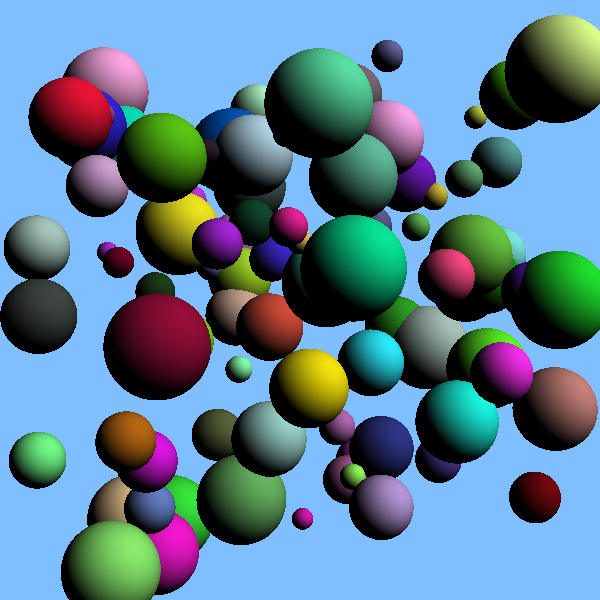
\includegraphics[scale=0.5]{randomspheres.png}}

      {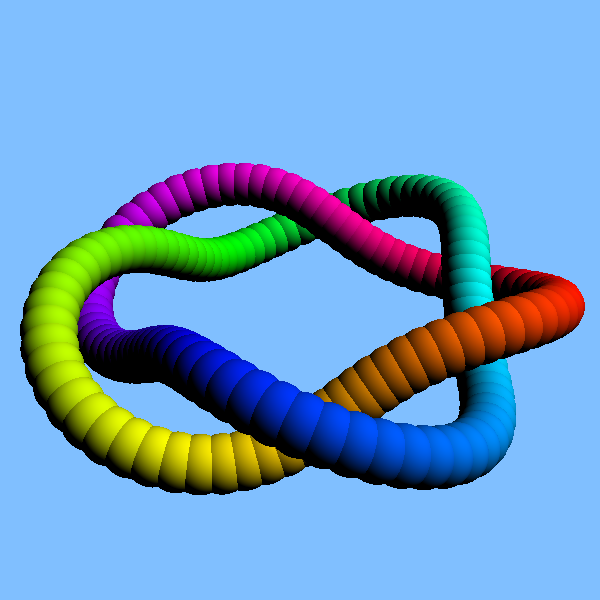
\includegraphics[scale=0.5]{ring01.png}}

      {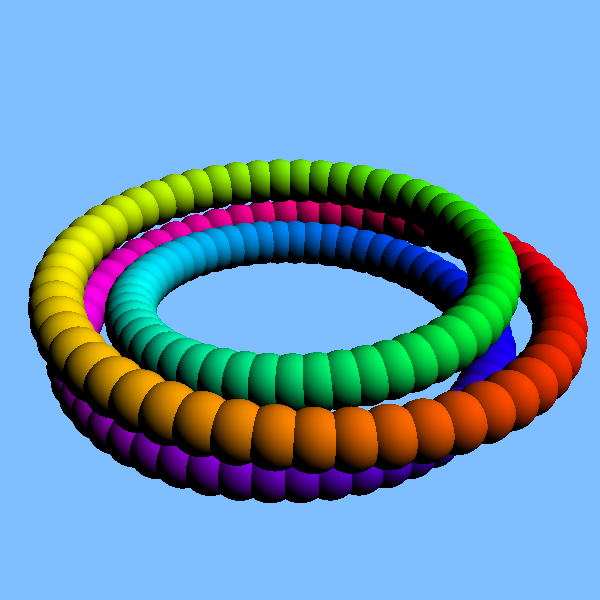
\includegraphics[scale=0.5]{ring03.png}}

      {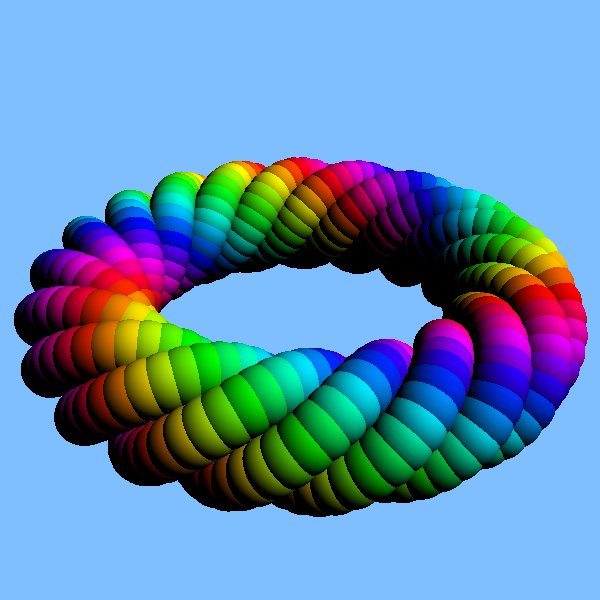
\includegraphics[scale=0.5]{ring02.png}}

\end{center}


\end{description}

\end{document}
